\chapter{NN plots}
\label{sec:appNNplots}

\section{Low mass splittings}

\subsection{Low level features}

\begin{figure}[H]
    \centering
    \begin{subfigure}[t!]{0.49\textwidth}
        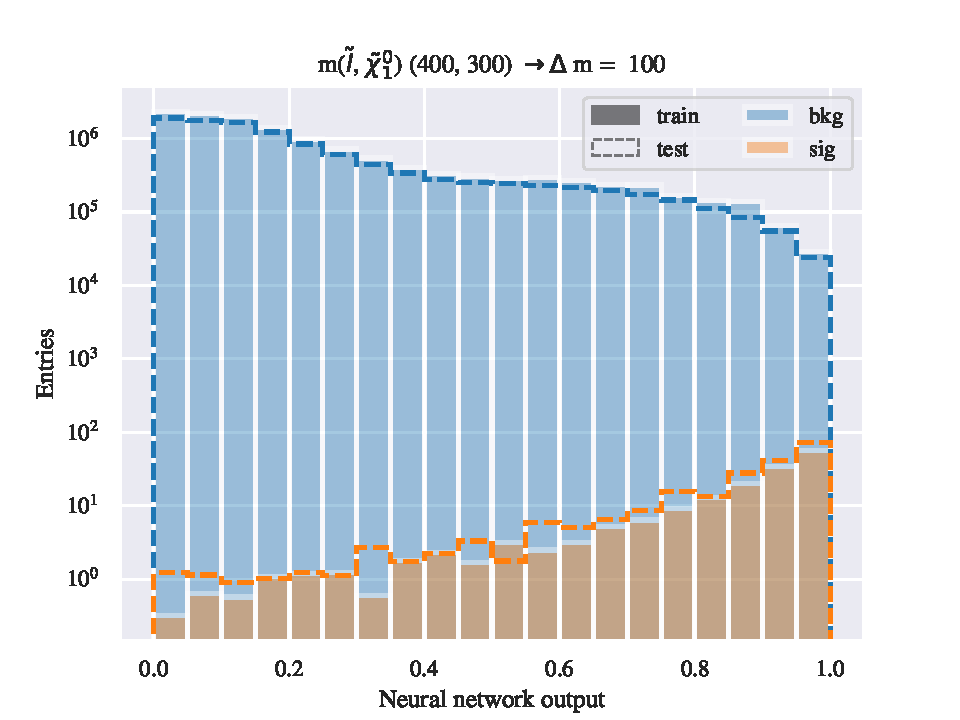
\includegraphics[width = \textwidth]{Figures/SlepSlep/ML/NN/Low_level/Low/scaled_train_test_395984.pdf}
        \caption{Direct slepton production.}
        \label{fig:}
    \end{subfigure}
    \begin{subfigure}[t!]{0.49\textwidth}
        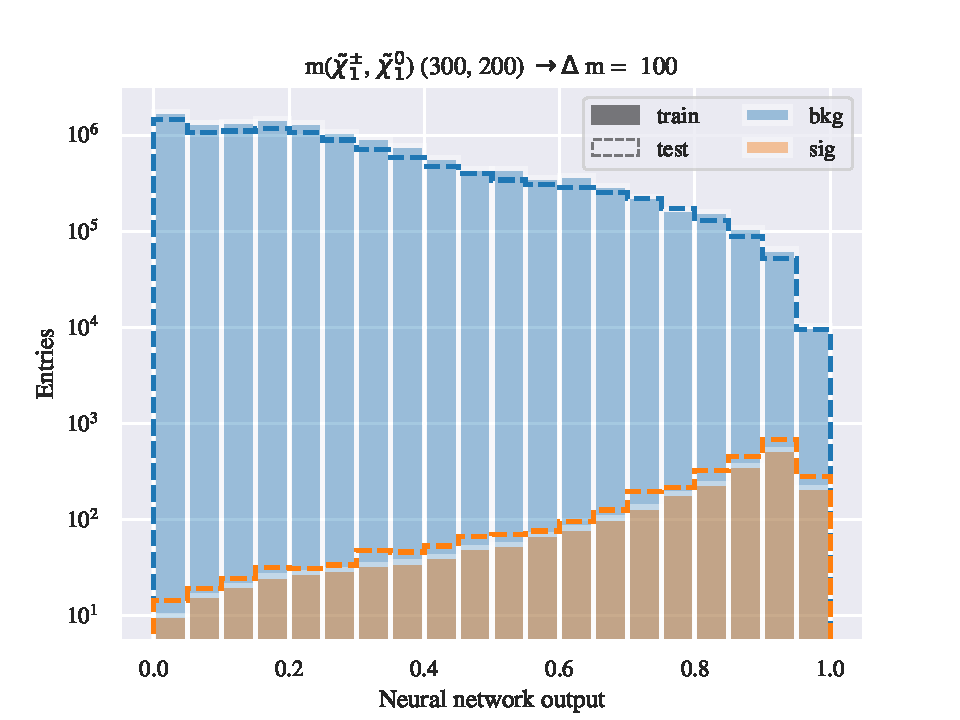
\includegraphics[width = \textwidth]{Figures/SlepSnu/NN/Low_level/Low/scaled_train_test_397115.pdf}
        \caption{Chargino production via $\Tilde{l}/\Tilde{\nu}$.}
        \label{fig:}
    \end{subfigure}    
    \begin{subfigure}[t!]{0.49\textwidth}
        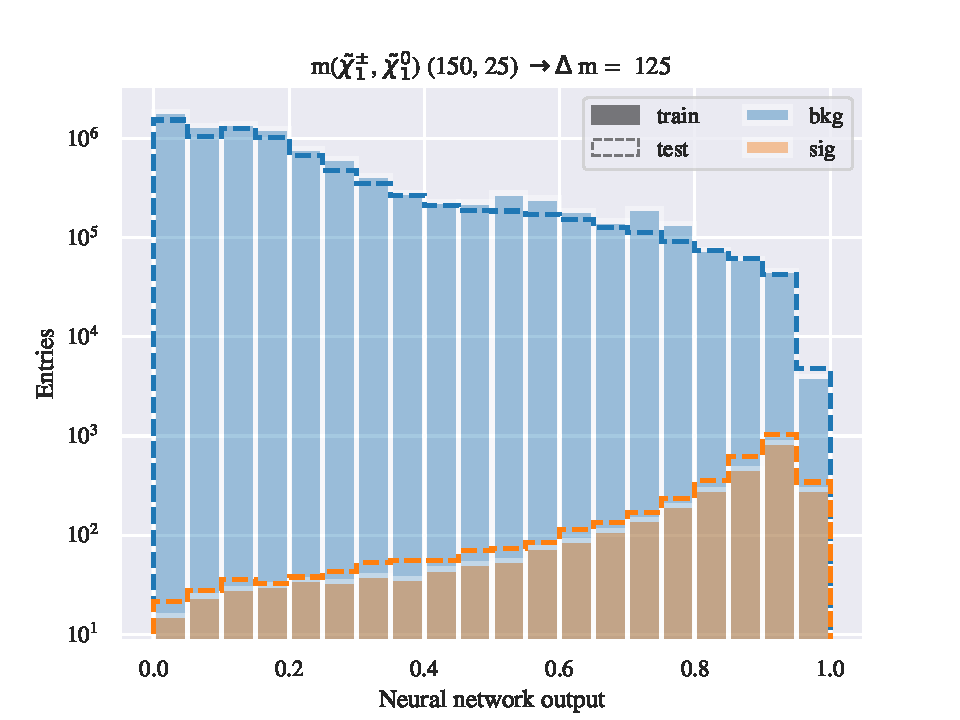
\includegraphics[width = \textwidth]{Figures/WW/NN/Low_level/Low/scaled_train_test_395268.pdf}
        \caption{Chargino production via $W^\pm$.}
        \label{fig:}
    \end{subfigure}
    \begin{subfigure}[t!]{0.49\textwidth}
        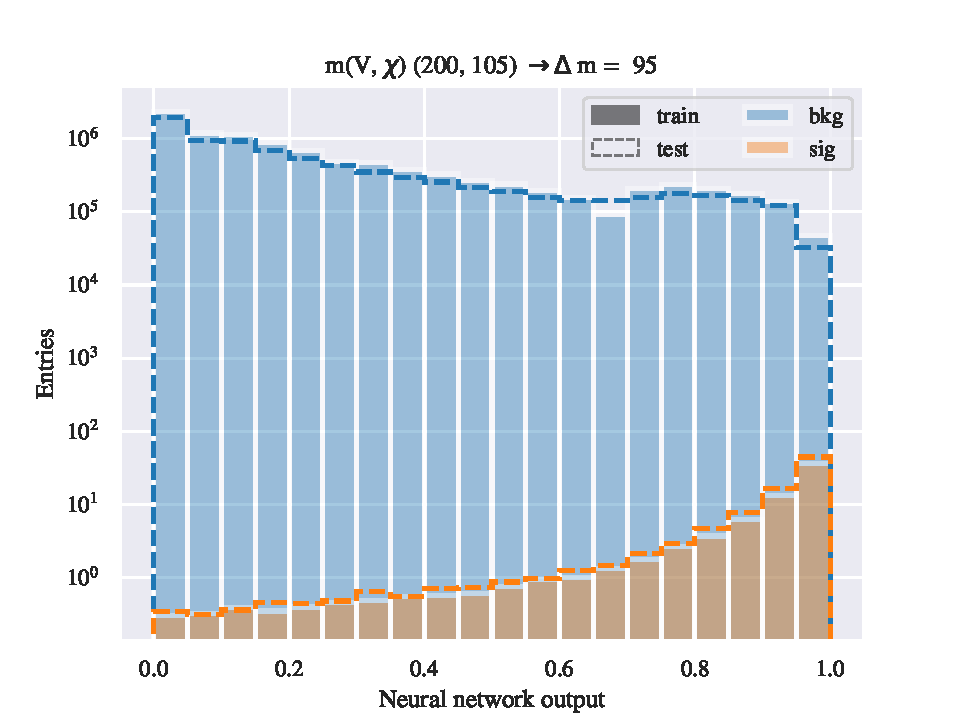
\includegraphics[width = \textwidth]{Figures/Mono_Z/ML/NN/Low_level/Low/scaled_train_test_310604.pdf}
        \caption{Mono-Z.}
        \label{fig:}
    \end{subfigure}
    \caption{Test vs train for low mass splittings done with the NN using low level features during training. Here the test set is scaled up to match the number of training events.}
    \label{fig:}
\end{figure}


\subsection{High level features}

\begin{figure}[H]
    \centering
    \begin{subfigure}[t!]{0.49\textwidth}
        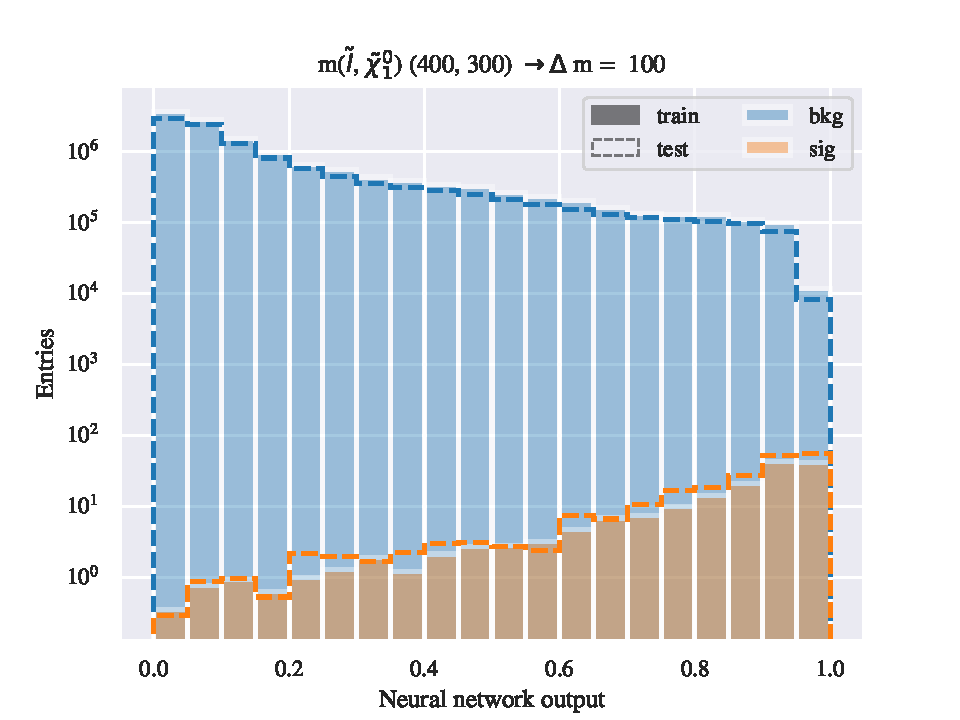
\includegraphics[width = \textwidth]{Figures/SlepSlep/ML/NN/High_level/Low/scaled_train_test_395984.pdf}
        \caption{Direct slepton production.}
        \label{fig:}
    \end{subfigure}
    \begin{subfigure}[t!]{0.49\textwidth}
        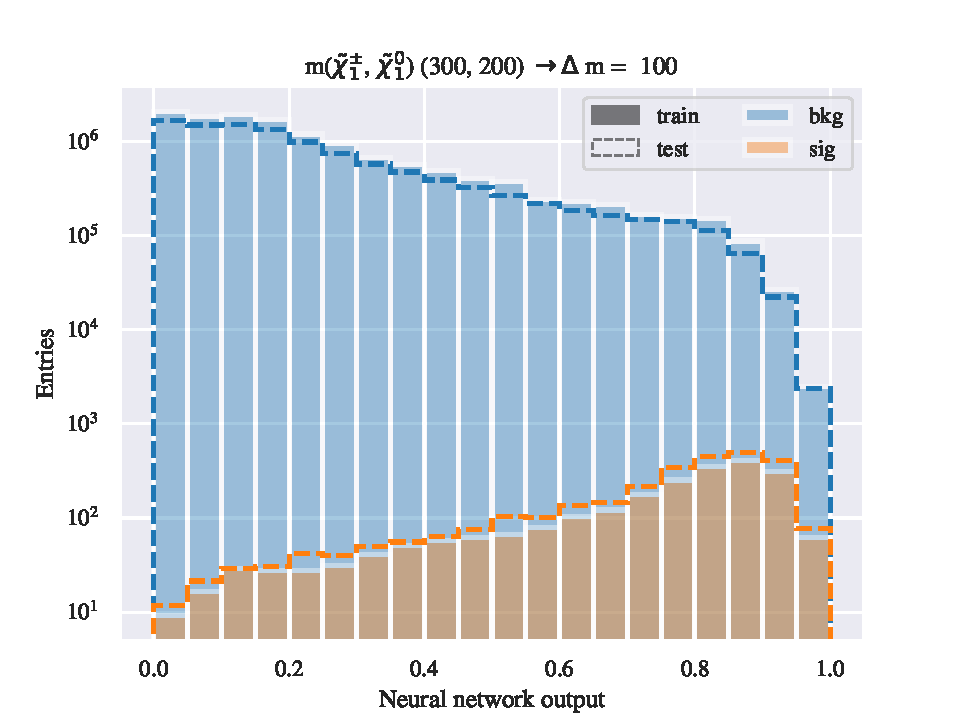
\includegraphics[width = \textwidth]{Figures/SlepSnu/NN/High_level/Low/scaled_train_test_397115.pdf}
        \caption{Chargino production via $\Tilde{l}/\Tilde{\nu}$.}
        \label{fig:}
    \end{subfigure}    
    \begin{subfigure}[t!]{0.49\textwidth}
        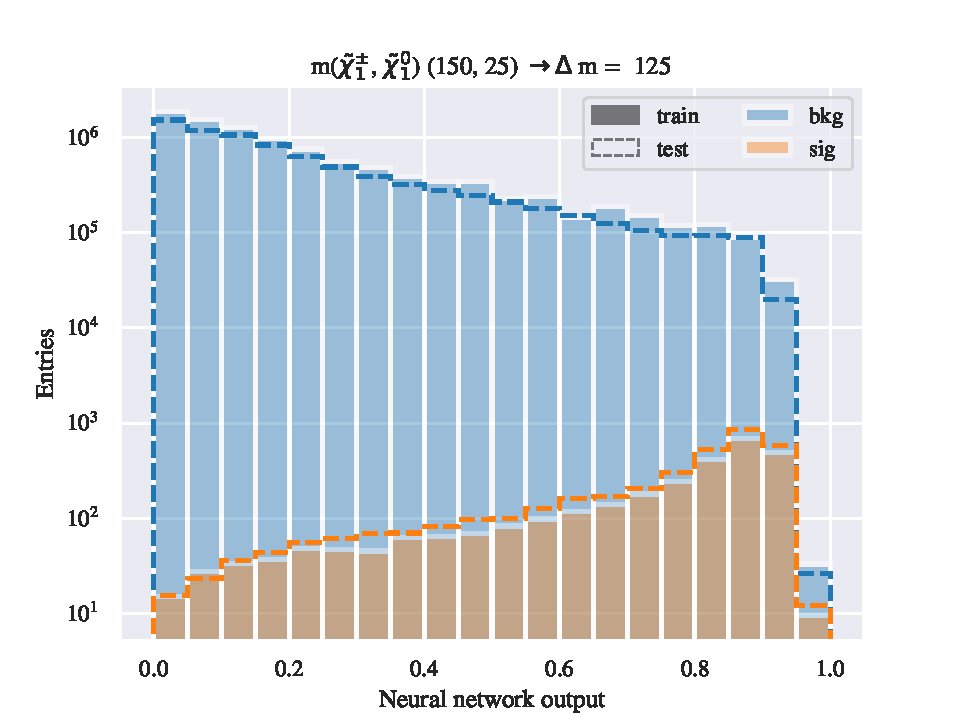
\includegraphics[width = \textwidth]{Figures/WW/NN/High_level/Low/scaled_train_test_395268.pdf}
        \caption{Chargino production via $W^\pm$.}
        \label{fig:}
    \end{subfigure}
    \begin{subfigure}[t!]{0.49\textwidth}
        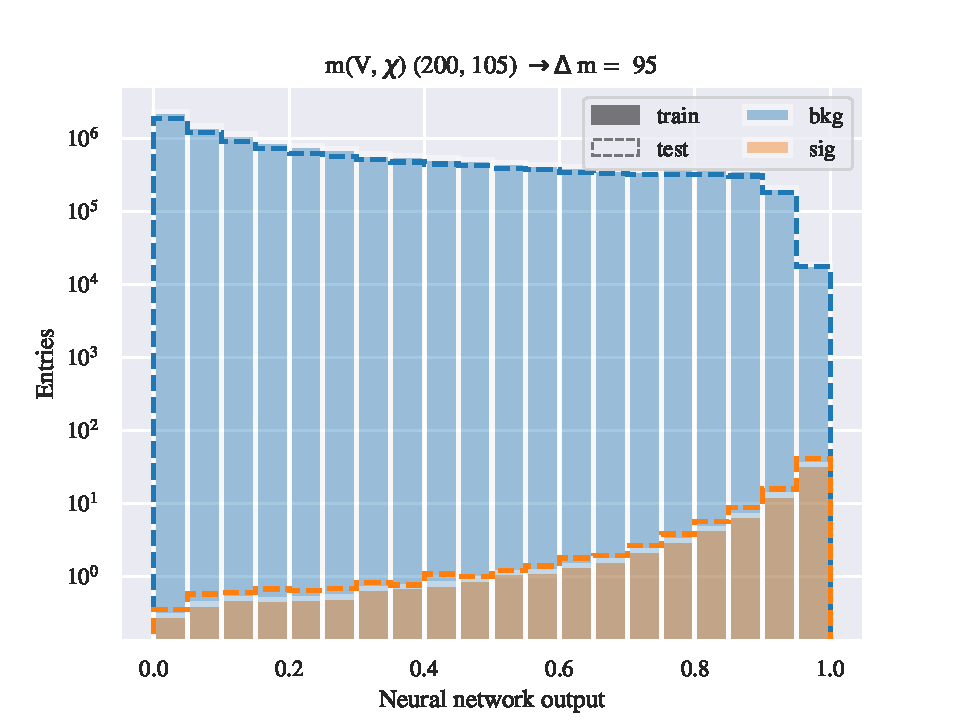
\includegraphics[width = \textwidth]{Figures/Mono_Z/ML/NN/High_level/Low/scaled_train_test_310604.pdf}
        \caption{Mono-Z.}
        \label{fig:}
    \end{subfigure}
    \caption{Test vs train for low mass splittings done with the NN using high level features during training. Here the test set is scaled up to match the number of training events.}
    \label{fig:}
\end{figure}





\section{Intermediate mass splittings}

\subsection{Low level features}

\begin{figure}[H]
    \centering
    \begin{subfigure}[t!]{0.49\textwidth}
        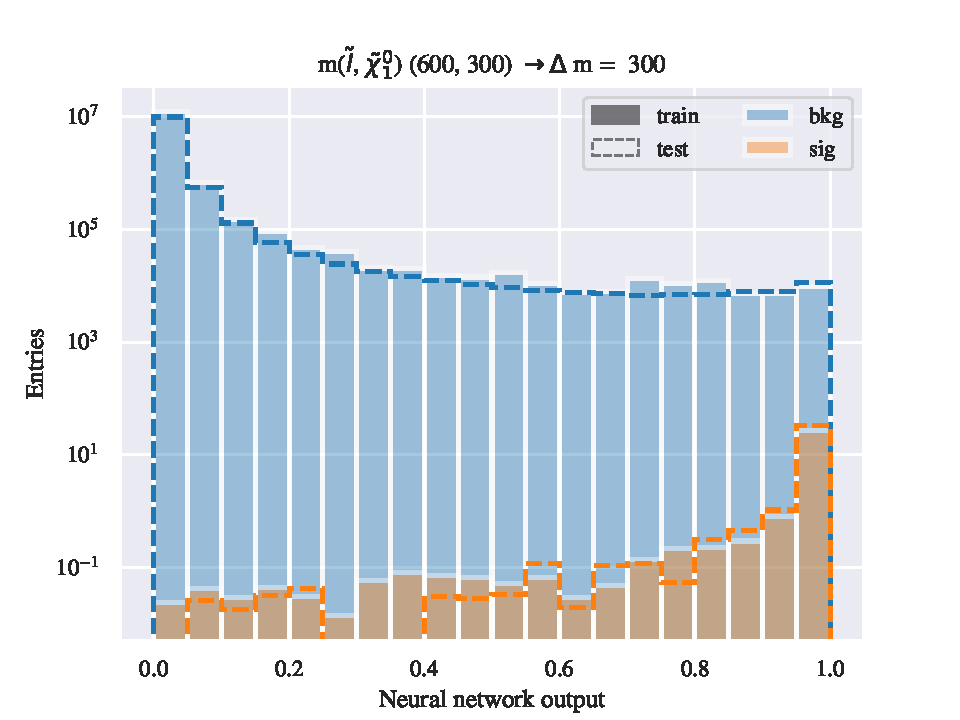
\includegraphics[width = \textwidth]{Figures/SlepSlep/ML/NN/Low_level/Inter/scaled_train_test_396014.pdf}
        \caption{Direct slepton production.}
        \label{fig:}
    \end{subfigure}
    \begin{subfigure}[t!]{0.49\textwidth}
        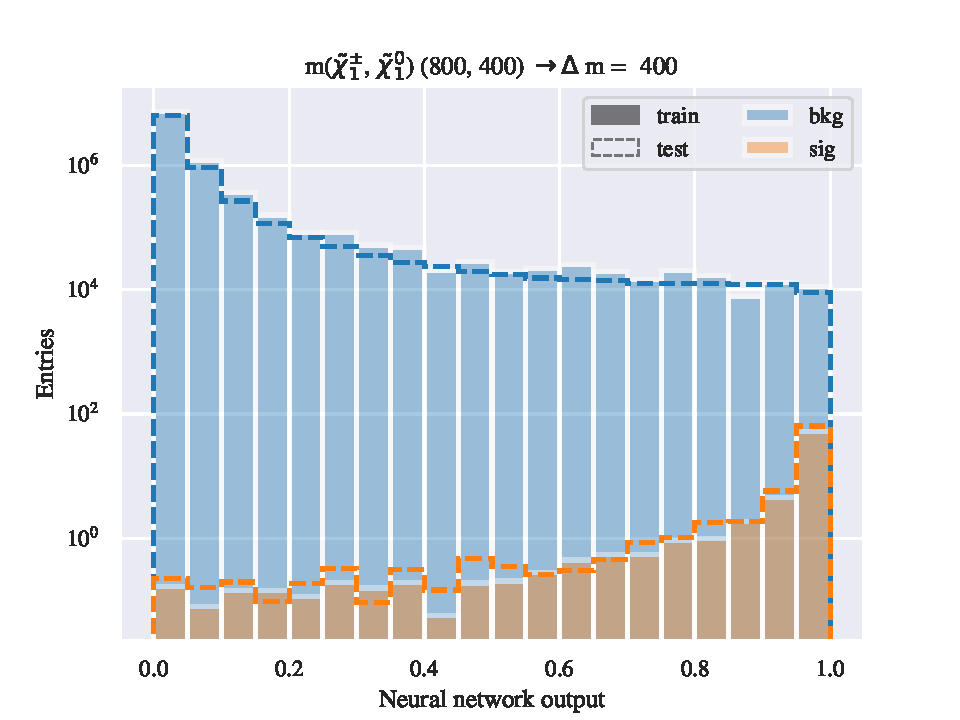
\includegraphics[width = \textwidth]{Figures/SlepSnu/NN/Low_level/Inter/scaled_train_test_397150.pdf}
        \caption{Chargino production via $\Tilde{l}/\Tilde{\nu}$.}
        \label{fig:}
    \end{subfigure}    
    \begin{subfigure}[t!]{0.49\textwidth}
        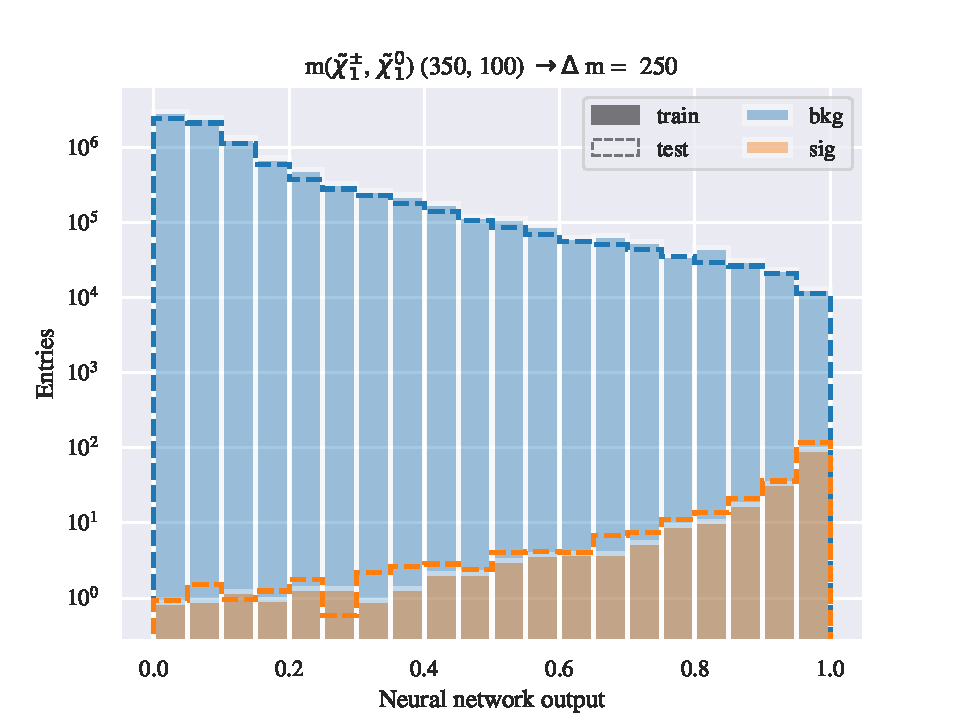
\includegraphics[width = \textwidth]{Figures/WW/NN/Low_level/Inter/scaled_train_test_395320.pdf}
        \caption{Chargino production via $W^\pm$.}
        \label{fig:}
    \end{subfigure}
    \begin{subfigure}[t!]{0.49\textwidth}
        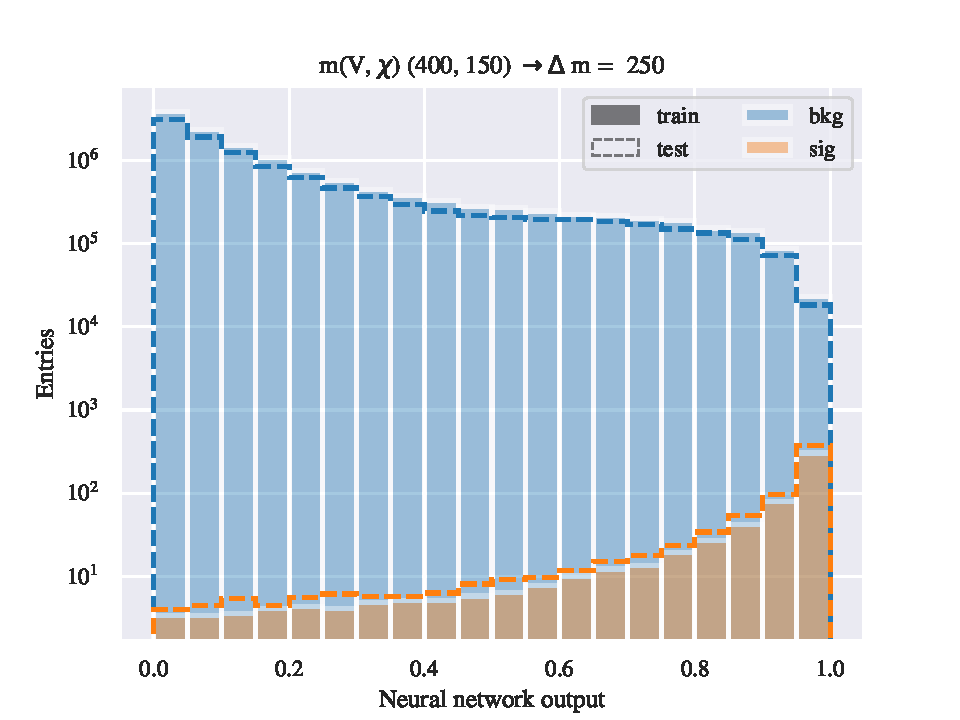
\includegraphics[width = \textwidth]{Figures/Mono_Z/ML/NN/Low_level/Inter/scaled_train_test_310613.pdf}
        \caption{Mono-Z.}
        \label{fig:}
    \end{subfigure}
    \caption{Test vs train for intermediate mass splittings done with the NN using low level features during training. Here the test set is scaled up to match the number of training events.}
    \label{fig:}
\end{figure}


\subsection{High level features}

\begin{figure}[H]
    \centering
    \begin{subfigure}[t!]{0.49\textwidth}
        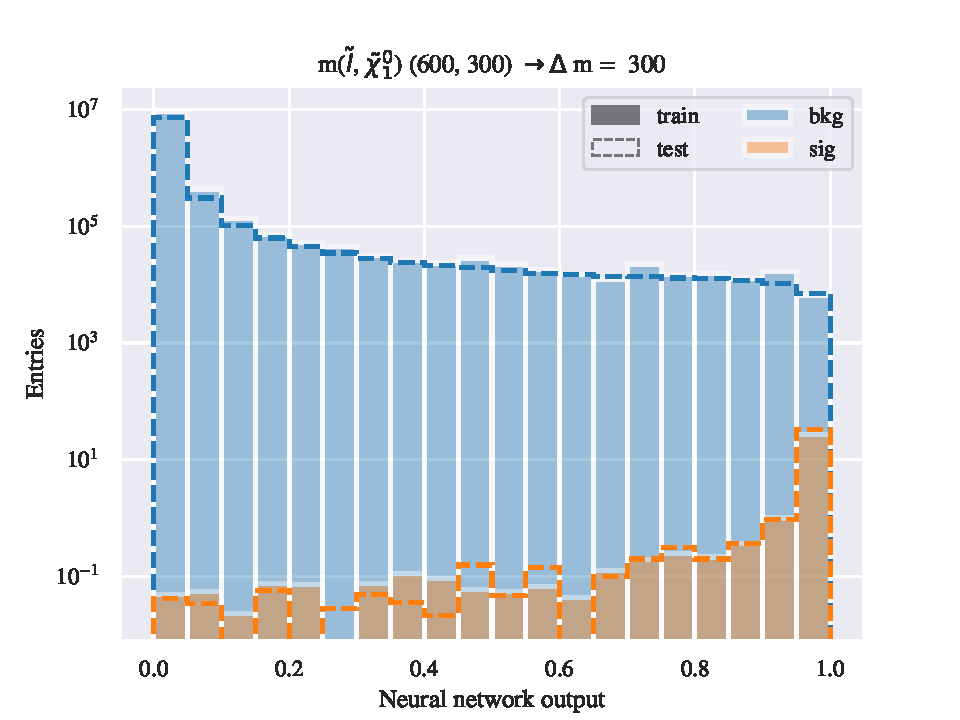
\includegraphics[width = \textwidth]{Figures/SlepSlep/ML/NN/High_level/Inter/scaled_train_test_396014.pdf}
        \caption{Direct slepton production.}
        \label{fig:}
    \end{subfigure}
    \begin{subfigure}[t!]{0.49\textwidth}
        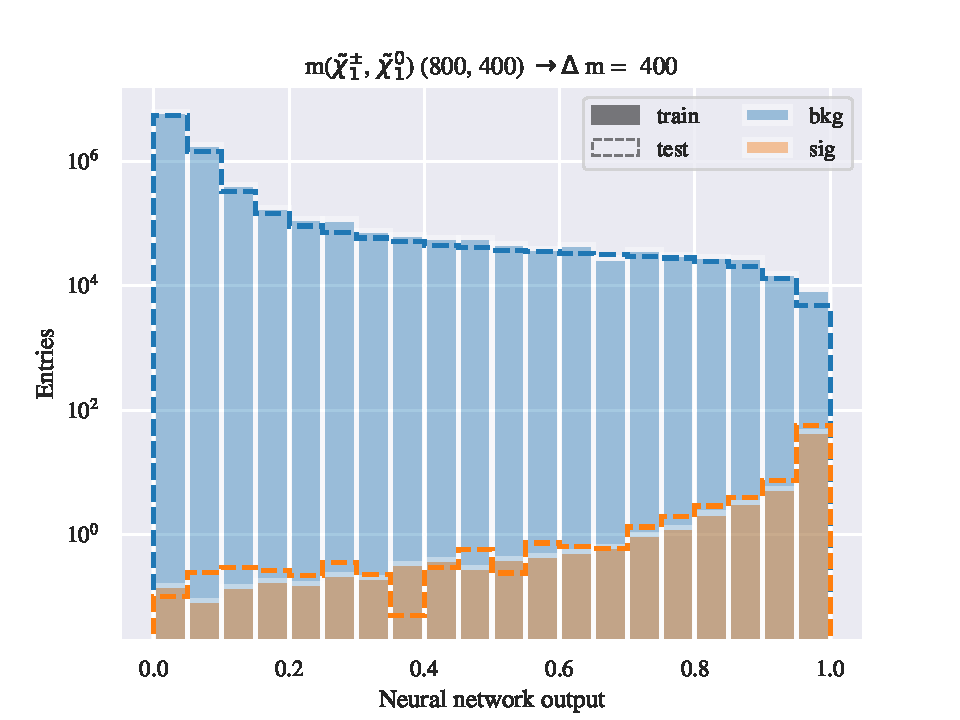
\includegraphics[width = \textwidth]{Figures/SlepSnu/NN/High_level/Inter/scaled_train_test_397150.pdf}
        \caption{Chargino production via $\Tilde{l}/\Tilde{\nu}$.}
        \label{fig:}
    \end{subfigure}    
    \begin{subfigure}[t!]{0.49\textwidth}
        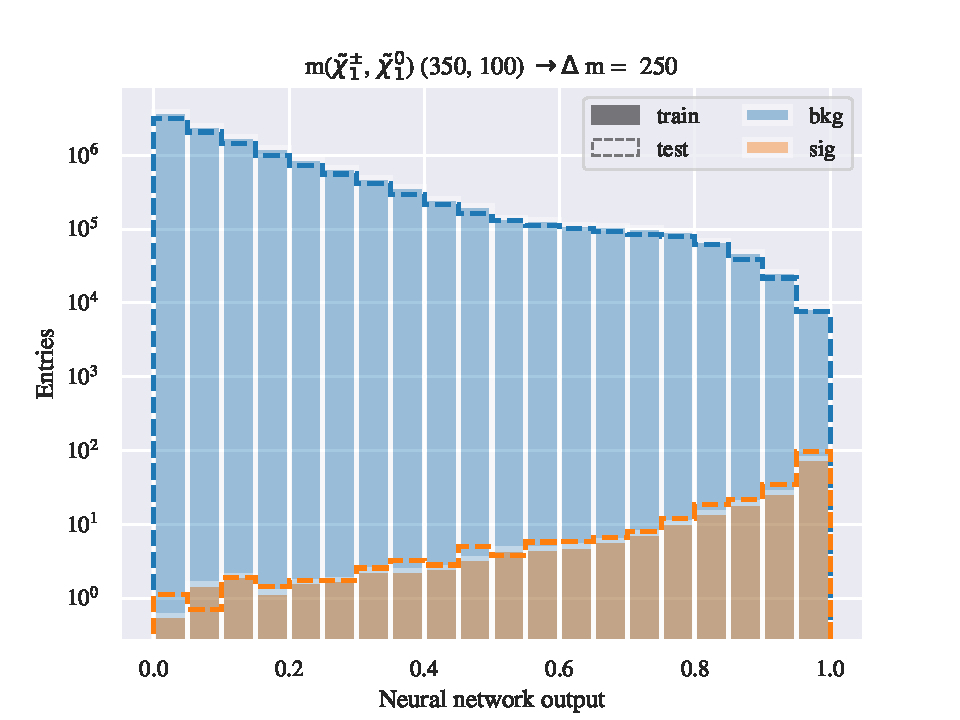
\includegraphics[width = \textwidth]{Figures/WW/NN/High_level/Inter/scaled_train_test_395320.pdf}
        \caption{Chargino production via $W^\pm$.}
        \label{fig:}
    \end{subfigure}
    \begin{subfigure}[t!]{0.49\textwidth}
        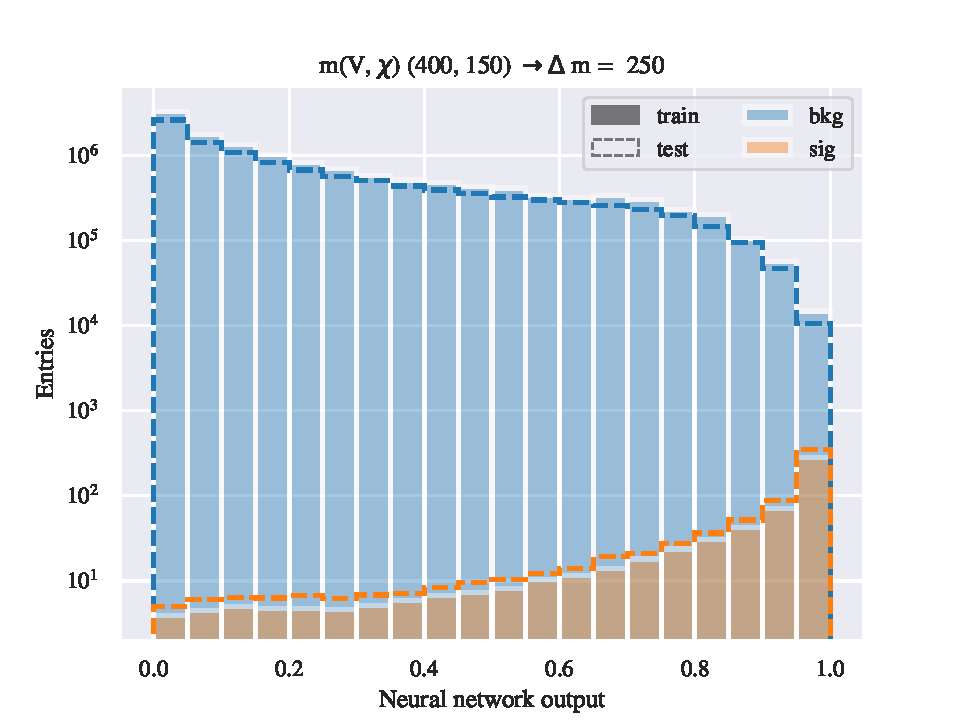
\includegraphics[width = \textwidth]{Figures/Mono_Z/ML/NN/High_level/Inter/scaled_train_test_310613.pdf}
        \caption{Mono-Z.}
        \label{fig:}
    \end{subfigure}
    \caption{Test vs train for intermediate mass splittings done with the NN using high level features during training. Here the test set is scaled up to match the number of training events.}
    \label{fig:}
\end{figure}






\section{High mass splittings}

\subsection{Low level features}

\begin{figure}[H]
    \centering
    \begin{subfigure}[t!]{0.49\textwidth}
        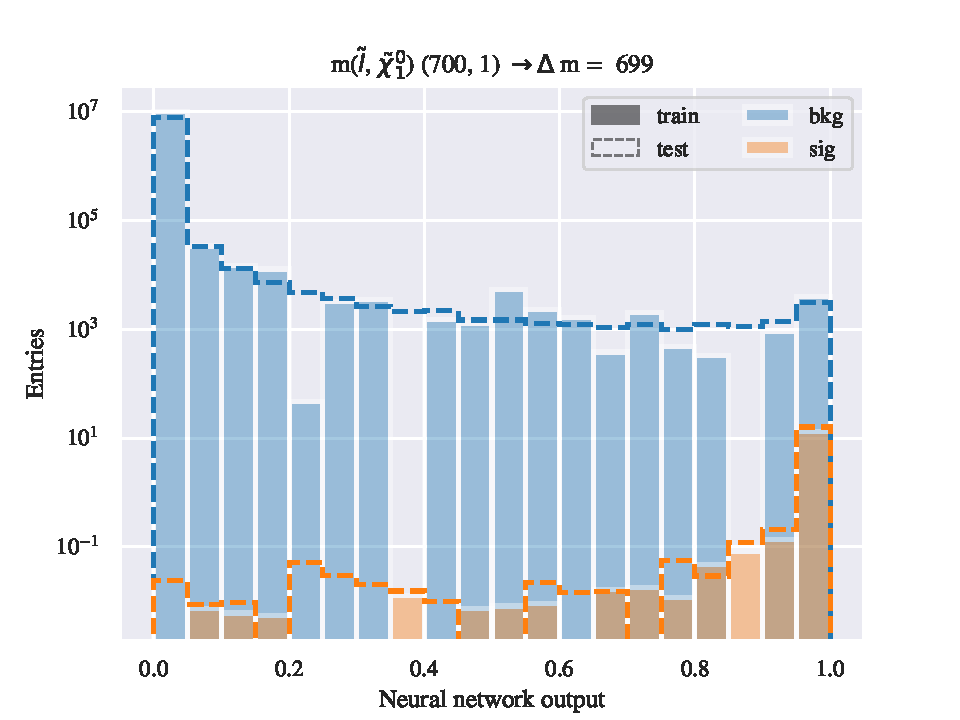
\includegraphics[width = \textwidth]{Figures/SlepSlep/ML/NN/Low_level/High/scaled_train_test_396033.pdf}
        \caption{Direct slepton production.}
        \label{fig:}
    \end{subfigure}
    \begin{subfigure}[t!]{0.49\textwidth}
        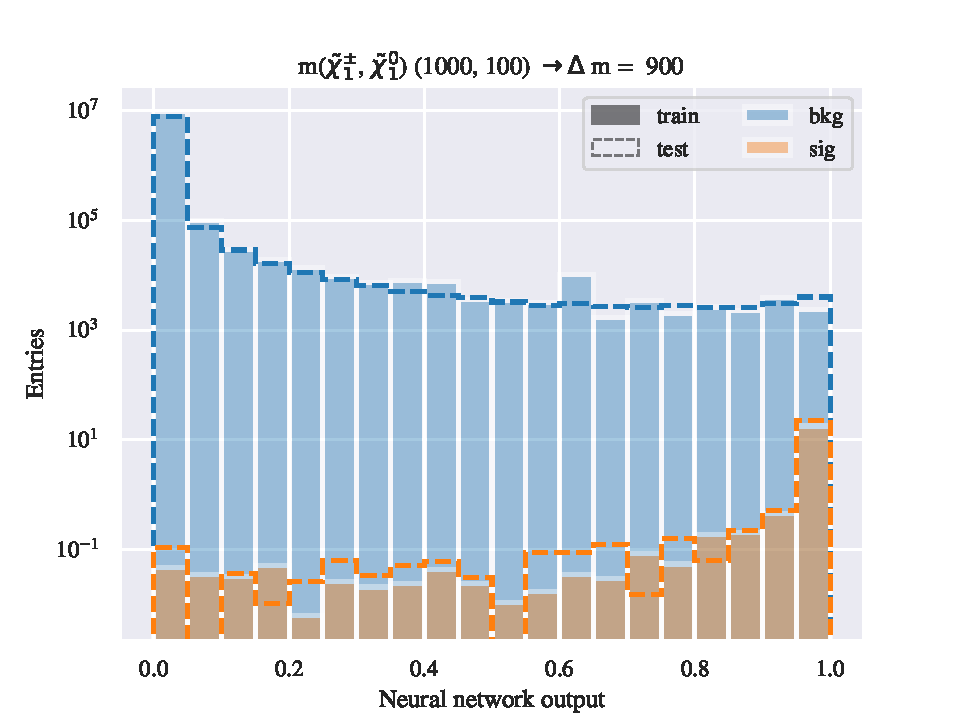
\includegraphics[width = \textwidth]{Figures/SlepSnu/NN/Low_level/High/scaled_train_test_397169.pdf}
        \caption{Chargino production via $\Tilde{l}/\Tilde{\nu}$.}
        \label{fig:}
    \end{subfigure}    
    \begin{subfigure}[t!]{0.49\textwidth}
        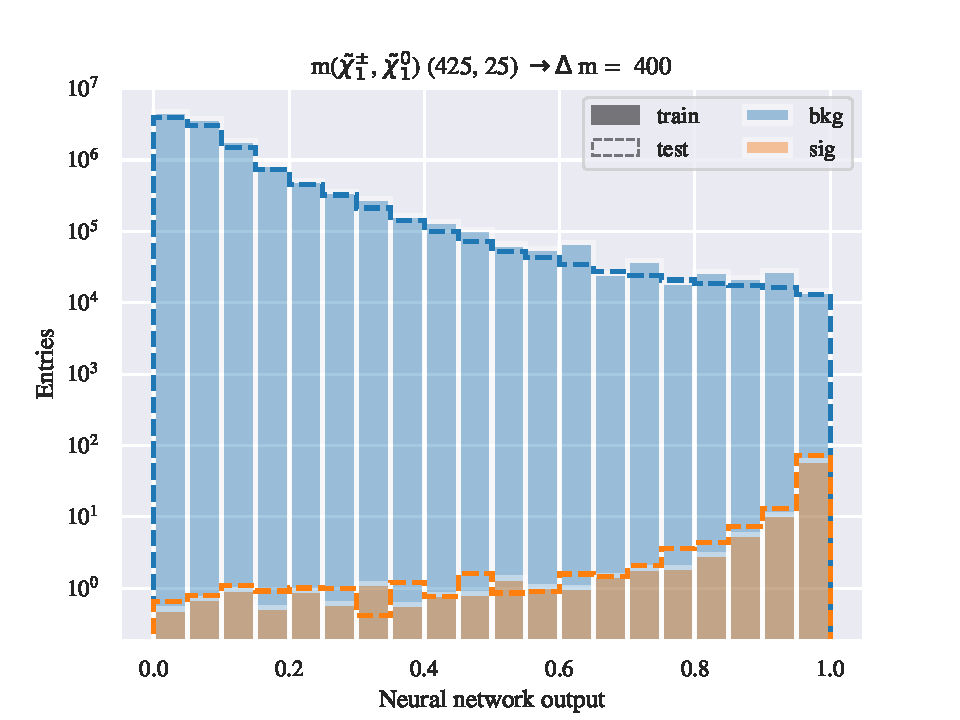
\includegraphics[width = \textwidth]{Figures/WW/NN/Low_level/High/scaled_train_test_395330.pdf}
        \caption{Chargino production via $W^\pm$.}
        \label{fig:}
    \end{subfigure}
    \begin{subfigure}[t!]{0.49\textwidth}
        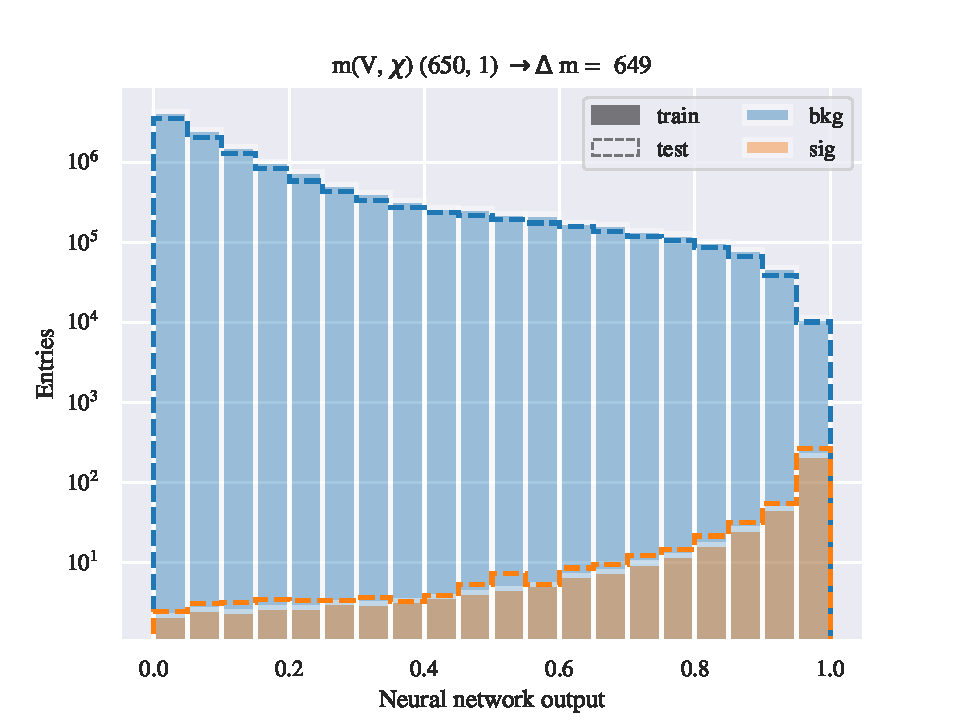
\includegraphics[width = \textwidth]{Figures/Mono_Z/ML/NN/Low_level/High/scaled_train_test_310617.pdf}
        \caption{Mono-Z.}
        \label{fig:}
    \end{subfigure}
    \caption{Test vs train for high mass splittings done with the NN using low level features during training. Here the test set is scaled up to match the number of training events.}
    \label{fig:}
\end{figure}


\subsection{High level features}

\begin{figure}[H]
    \centering
    \begin{subfigure}[t!]{0.49\textwidth}
        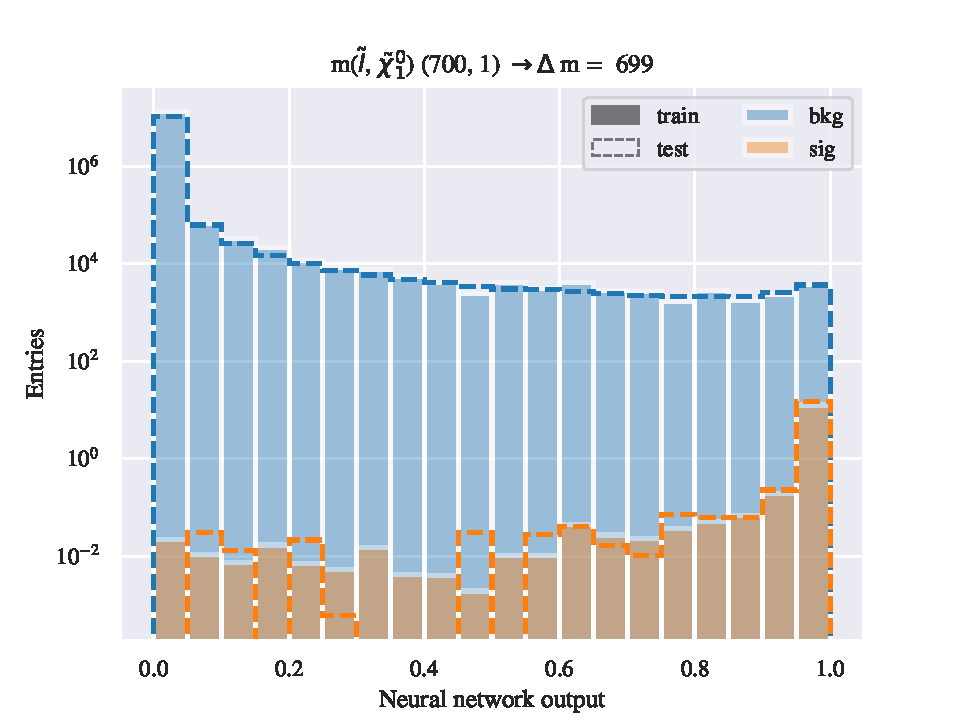
\includegraphics[width = \textwidth]{Figures/SlepSlep/ML/NN/High_level/High/scaled_train_test_396033.pdf}
        \caption{Direct slepton production.}
        \label{fig:}
    \end{subfigure}
    \begin{subfigure}[t!]{0.49\textwidth}
        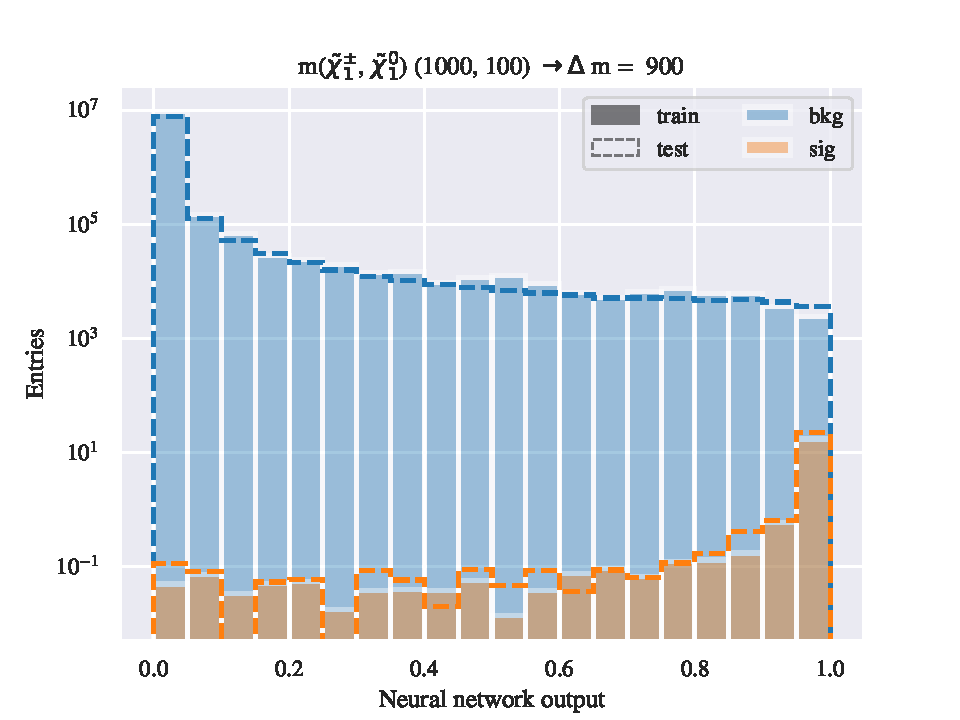
\includegraphics[width = \textwidth]{Figures/SlepSnu/NN/High_level/High/scaled_train_test_397169.pdf}
        \caption{Chargino production via $\Tilde{l}/\Tilde{\nu}$.}
        \label{fig:}
    \end{subfigure}    
    \begin{subfigure}[t!]{0.49\textwidth}
        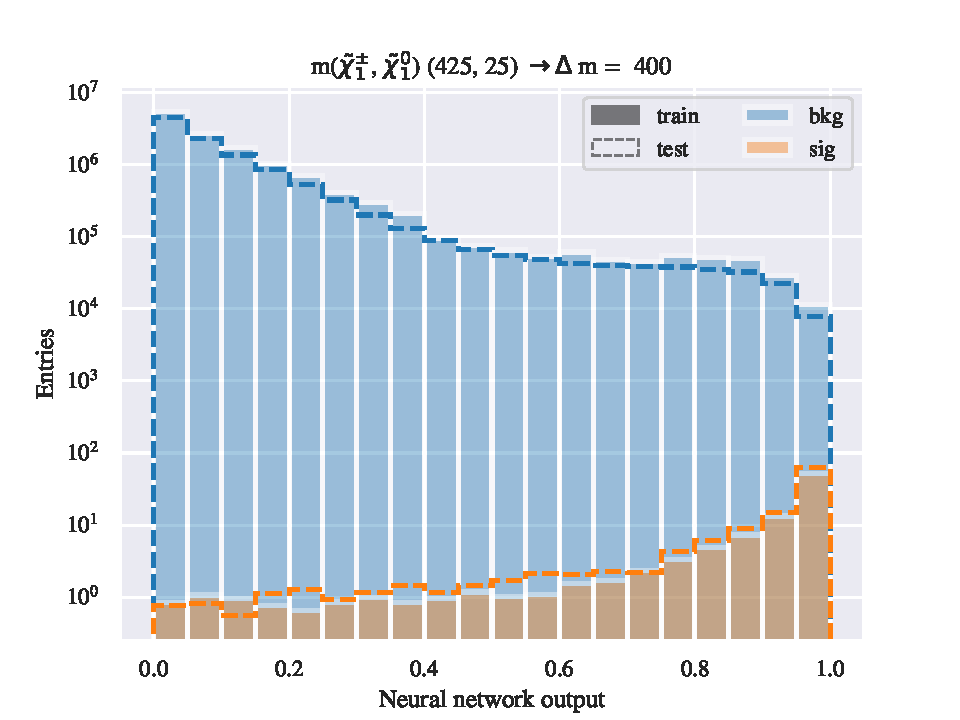
\includegraphics[width = \textwidth]{Figures/WW/NN/High_level/High/scaled_train_test_395330.pdf}
        \caption{Chargino production via $W^\pm$.}
        \label{fig:}
    \end{subfigure}
    \begin{subfigure}[t!]{0.49\textwidth}
        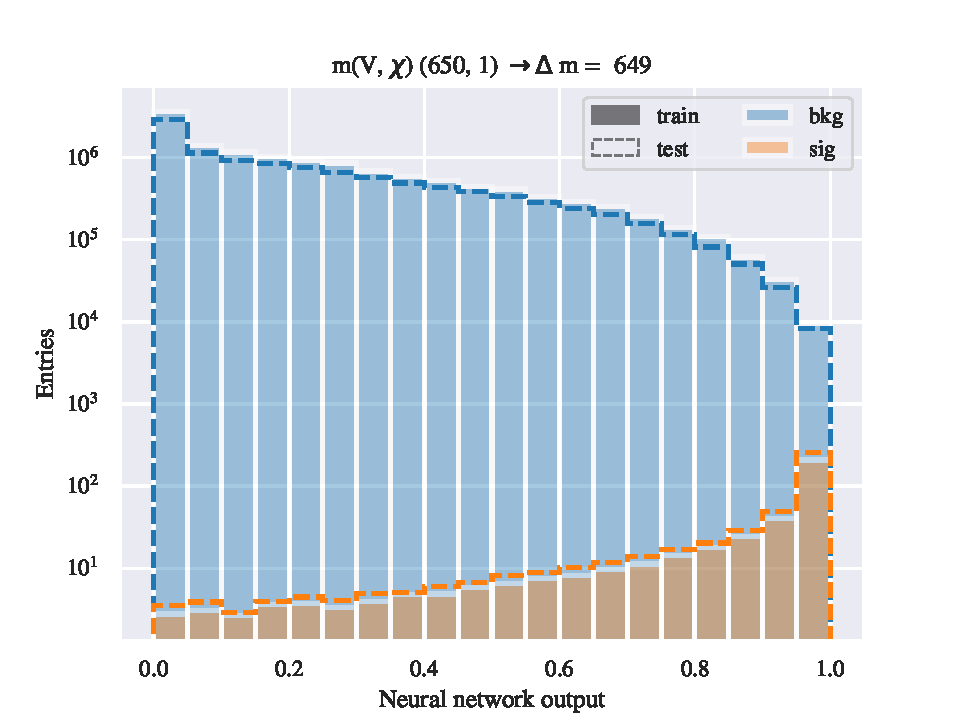
\includegraphics[width = \textwidth]{Figures/Mono_Z/ML/NN/High_level/High/scaled_train_test_310617.pdf}
        \caption{Mono-Z.}
        \label{fig:}
    \end{subfigure}
    \caption{Test vs train for high mass splittings done with the NN using high level features during training. Here the test set is scaled up to match the number of training events.}
    \label{fig:}
\end{figure}





\section{Stacked background with data}

\subsection{Low level features}

\begin{figure}[H]
    \centering
    \begin{subfigure}[t!]{0.49\textwidth}
        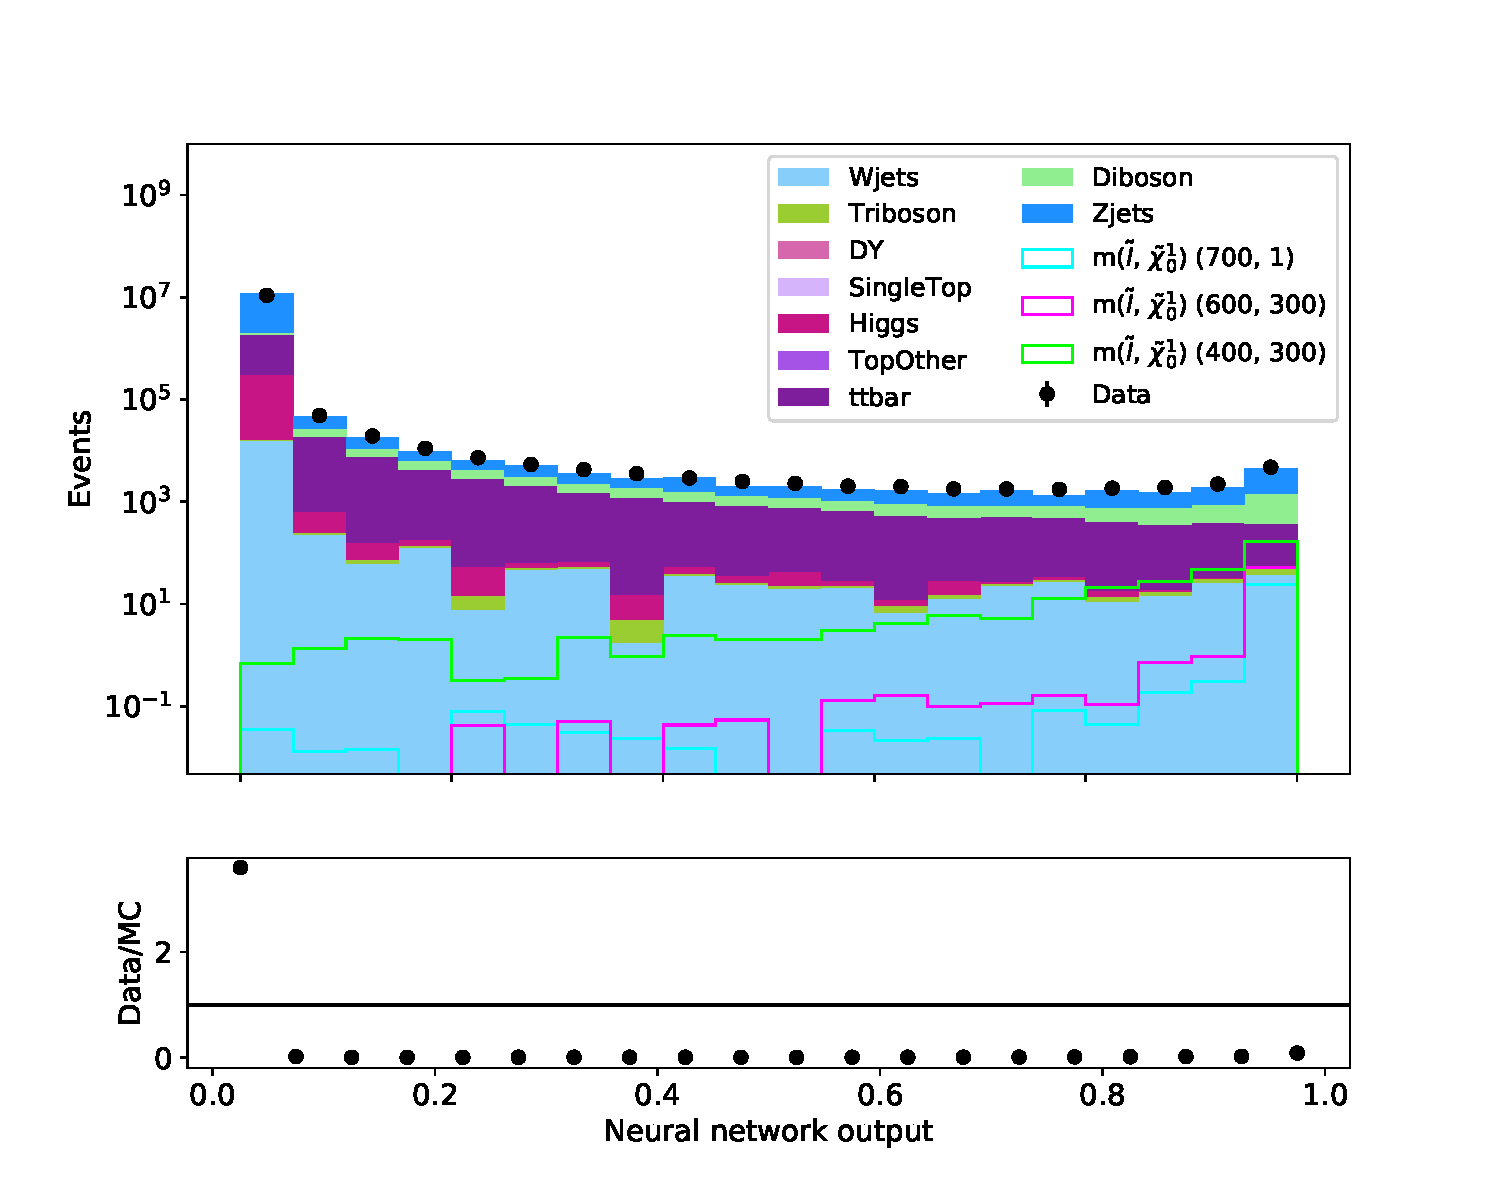
\includegraphics[width = \textwidth]{Figures/Stacked/stackedplot_NN_Low_level_slepslep.pdf}
        \caption{Direct slepton production.}
        \label{fig:}
    \end{subfigure}
    \begin{subfigure}[t!]{0.49\textwidth}
        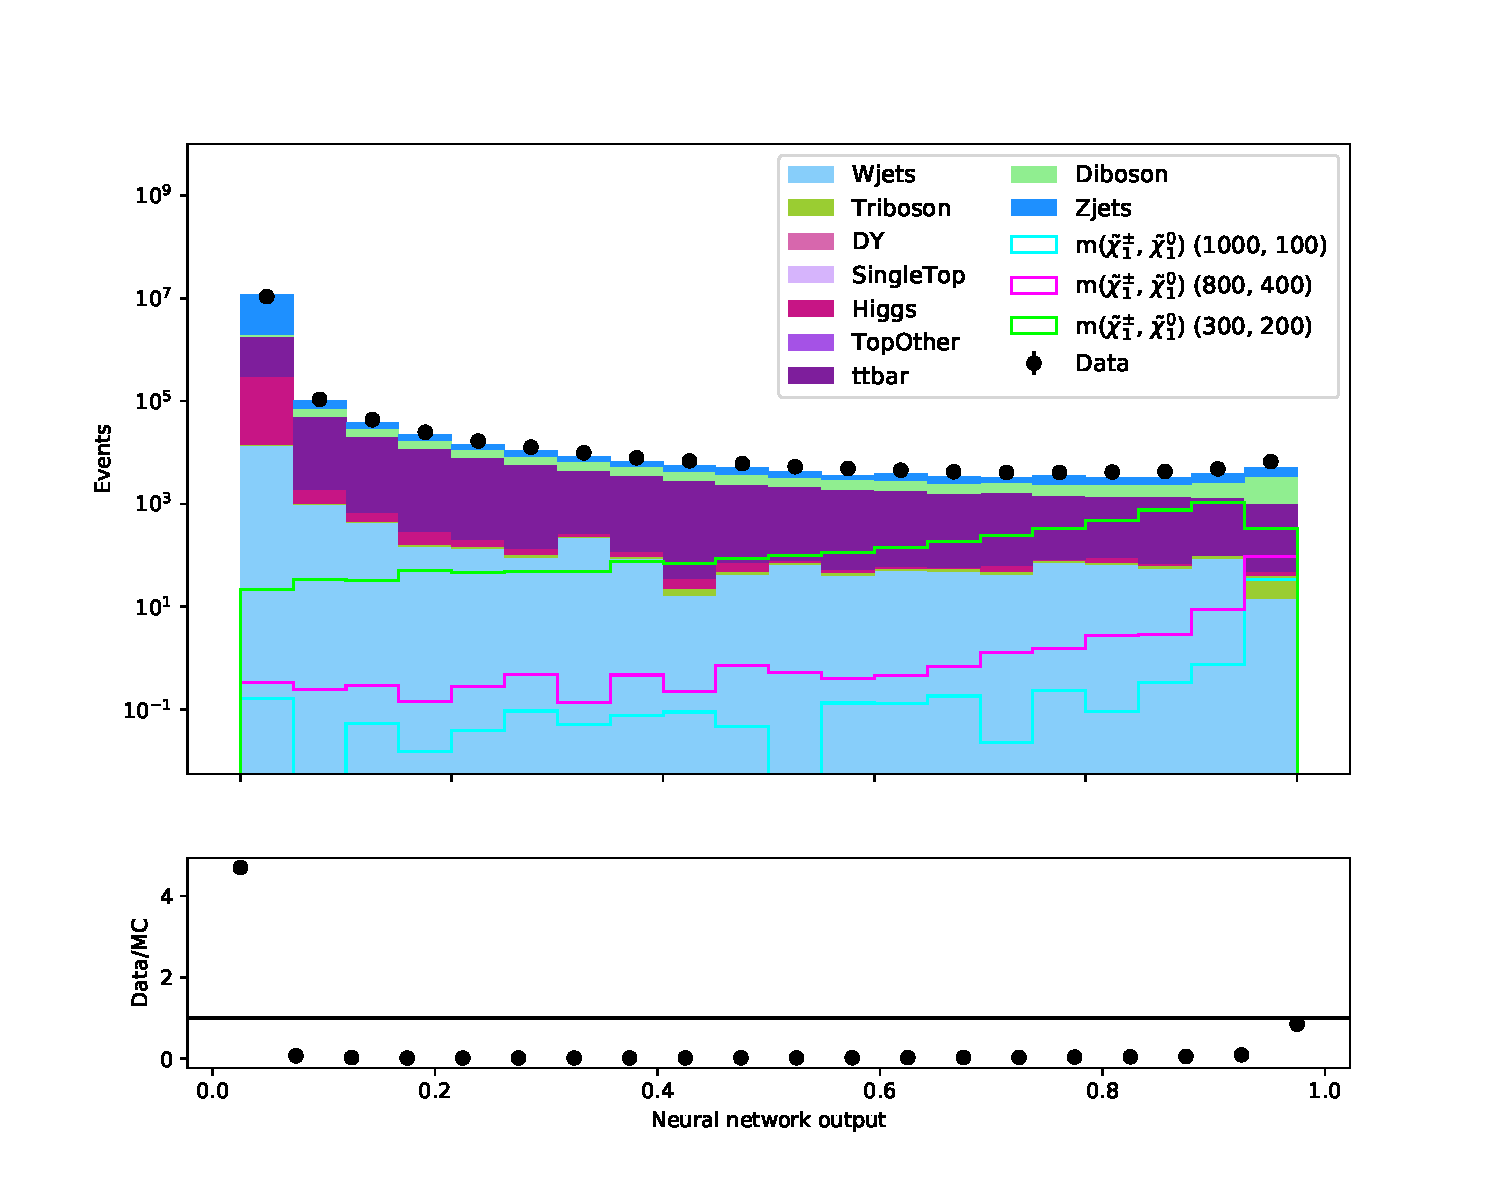
\includegraphics[width = \textwidth]{Figures/Stacked/stackedplot_NN_Low_level_slepsnu.pdf}
        \caption{Chargino production via $\Tilde{l}/\Tilde{\nu}$.}
        \label{fig:}
    \end{subfigure}      
    \begin{subfigure}[t!]{0.49\textwidth}
        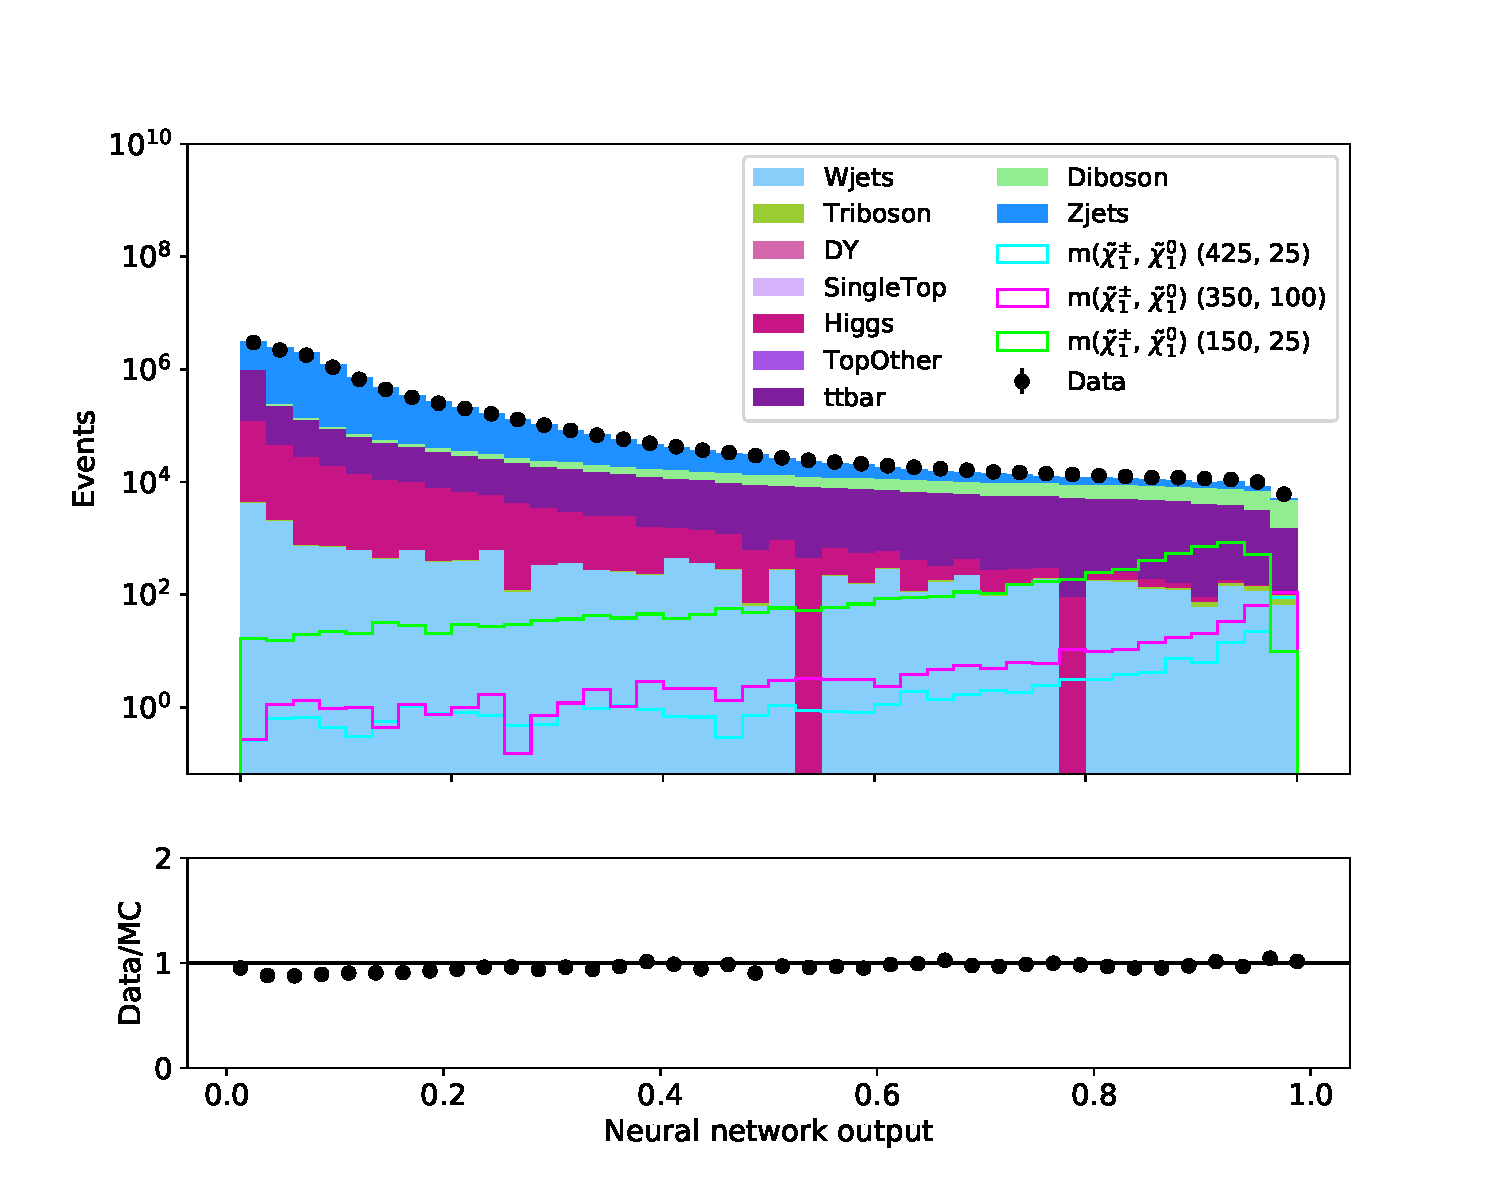
\includegraphics[width = \textwidth]{Figures/Stacked/stackedplot_NN_Low_level_WW.pdf}
        \caption{Chargino production via $W^\pm$.}
        \label{fig:}
    \end{subfigure}
    \begin{subfigure}[t!]{0.49\textwidth}
        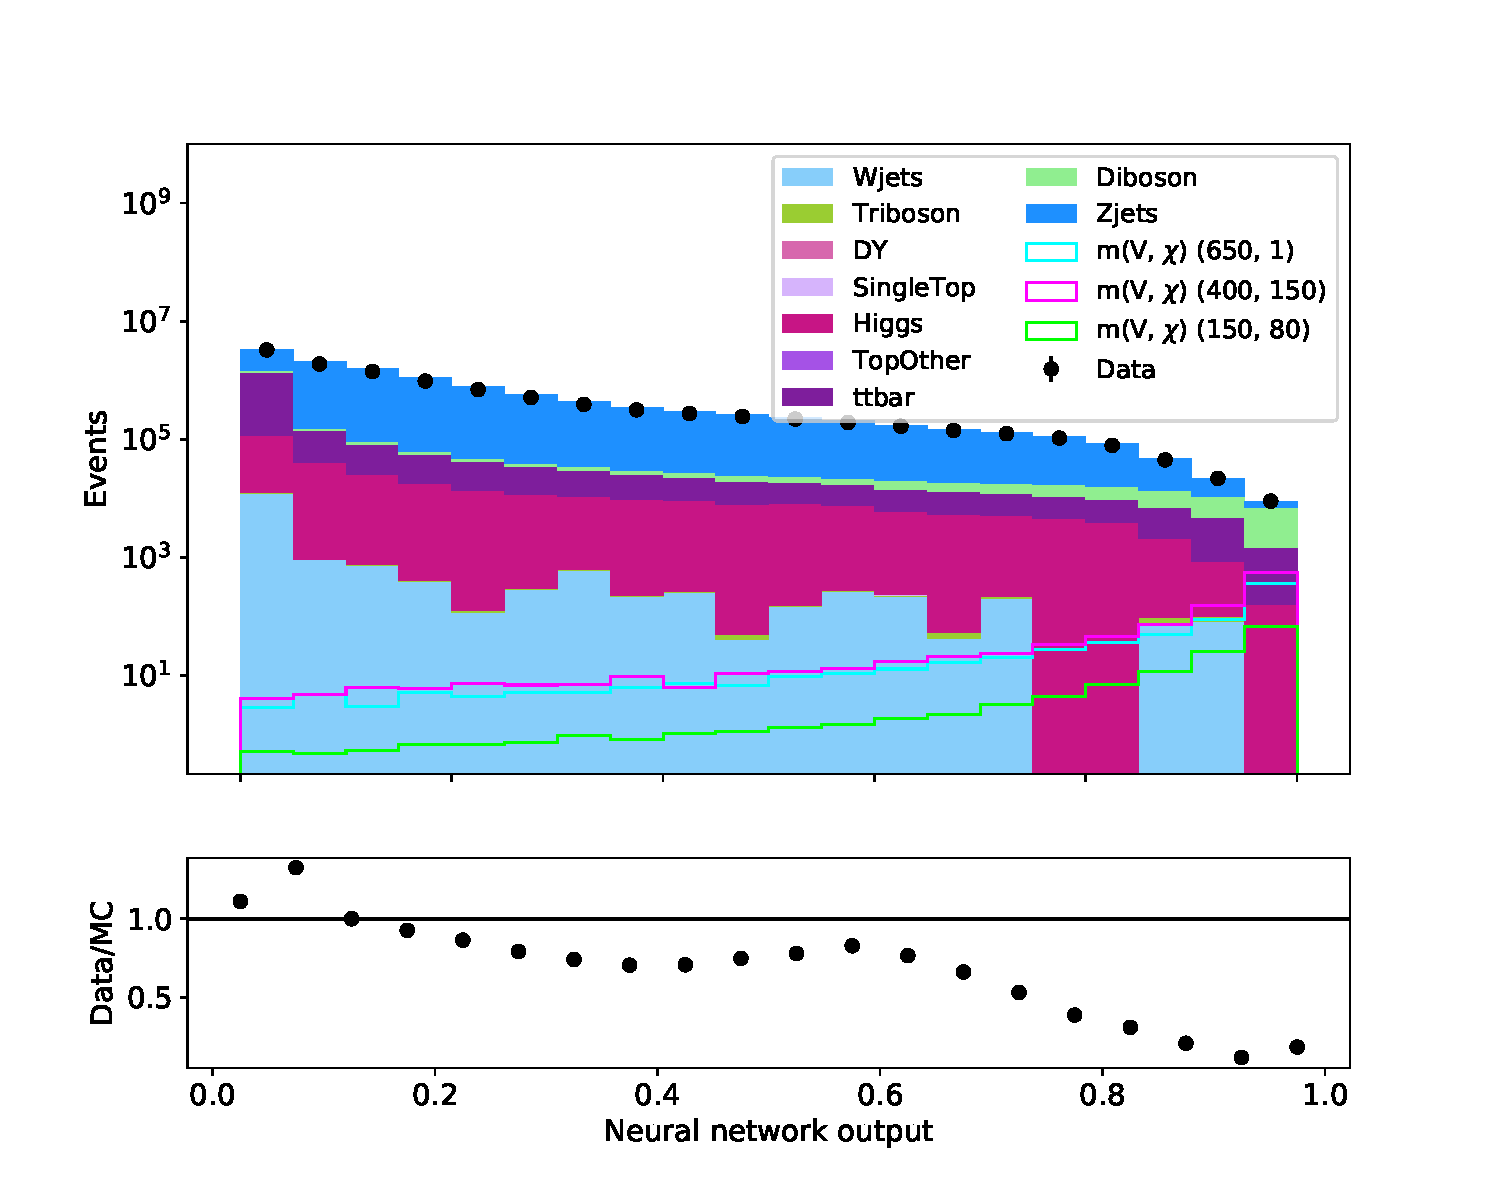
\includegraphics[width = \textwidth]{Figures/Stacked/stackedplot_NN_Low_level_monoZ.pdf}
        \caption{Mono-Z.}
        \label{fig:}
    \end{subfigure}
    \caption{Test vs train for low mass splittings done with the NN using low level features during training. Here the test set is scaled up to match the number of training events.}
    \label{fig:}
\end{figure}


\subsection{High level features}

\begin{figure}[H]
    \centering
    \begin{subfigure}[t!]{0.49\textwidth}
        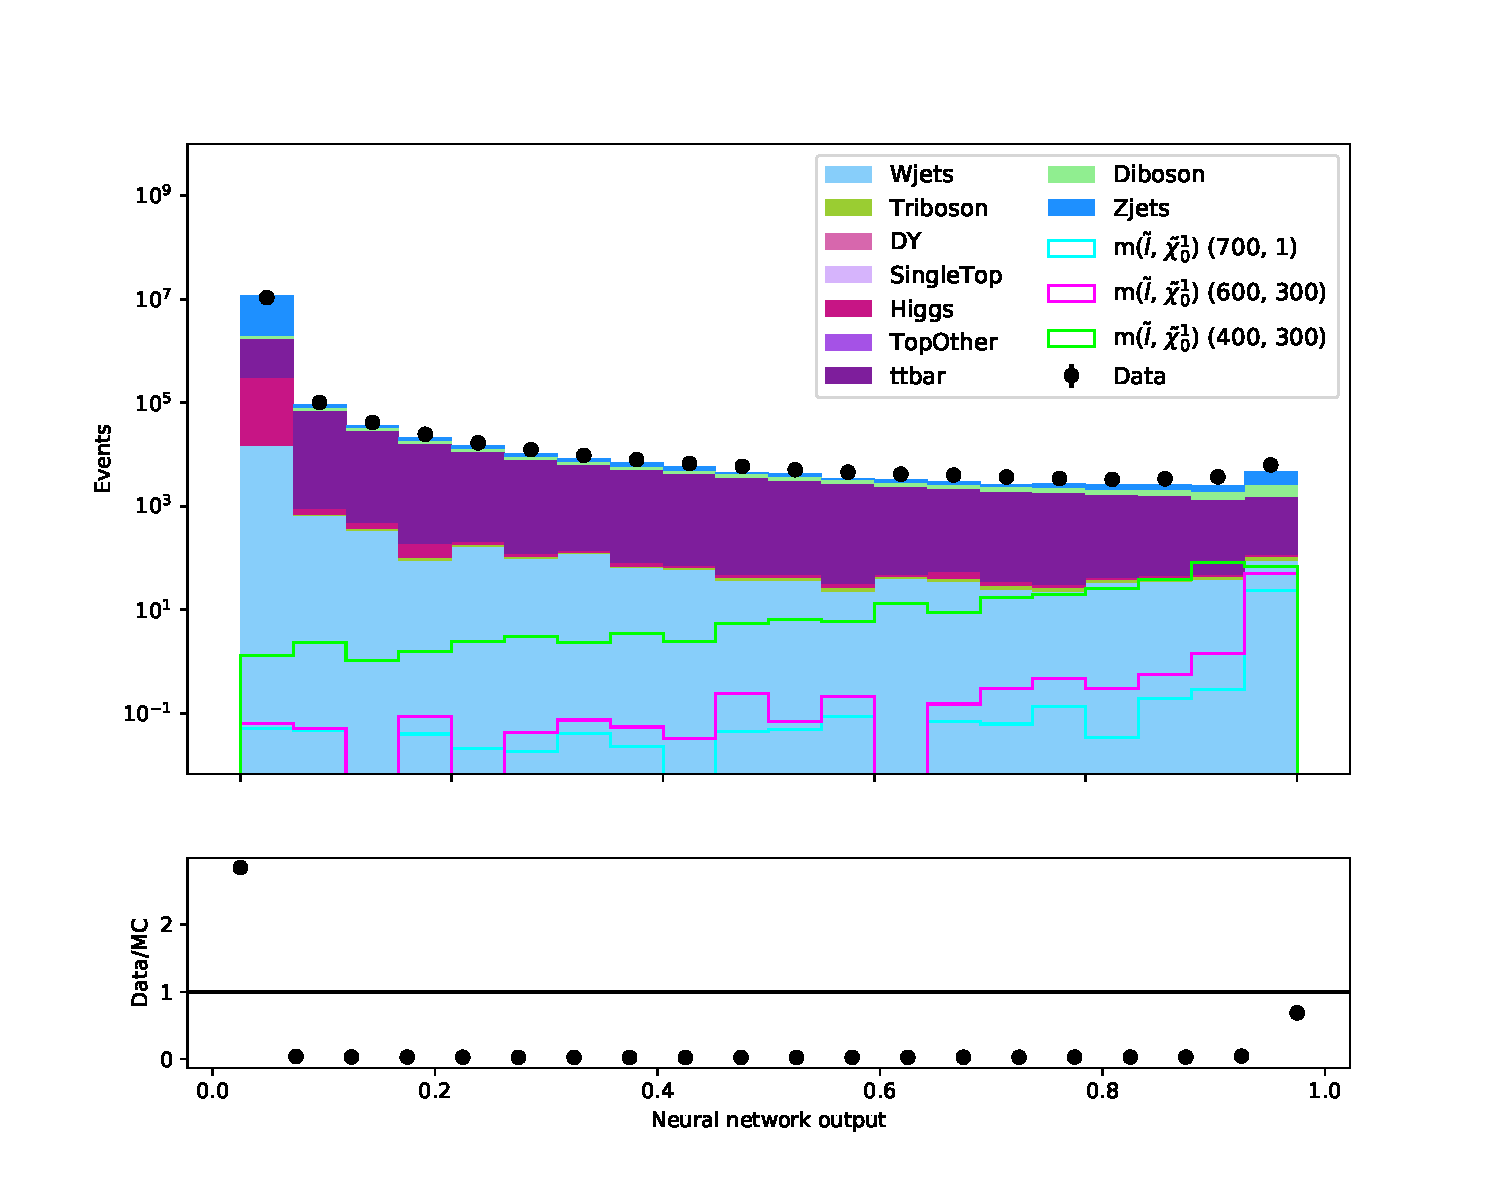
\includegraphics[width = \textwidth]{Figures/Stacked/stackedplot_NN_High_level_slepslep.pdf}
        \caption{Direct slepton production.}
        \label{fig:}
    \end{subfigure}
    \begin{subfigure}[t!]{0.49\textwidth}
        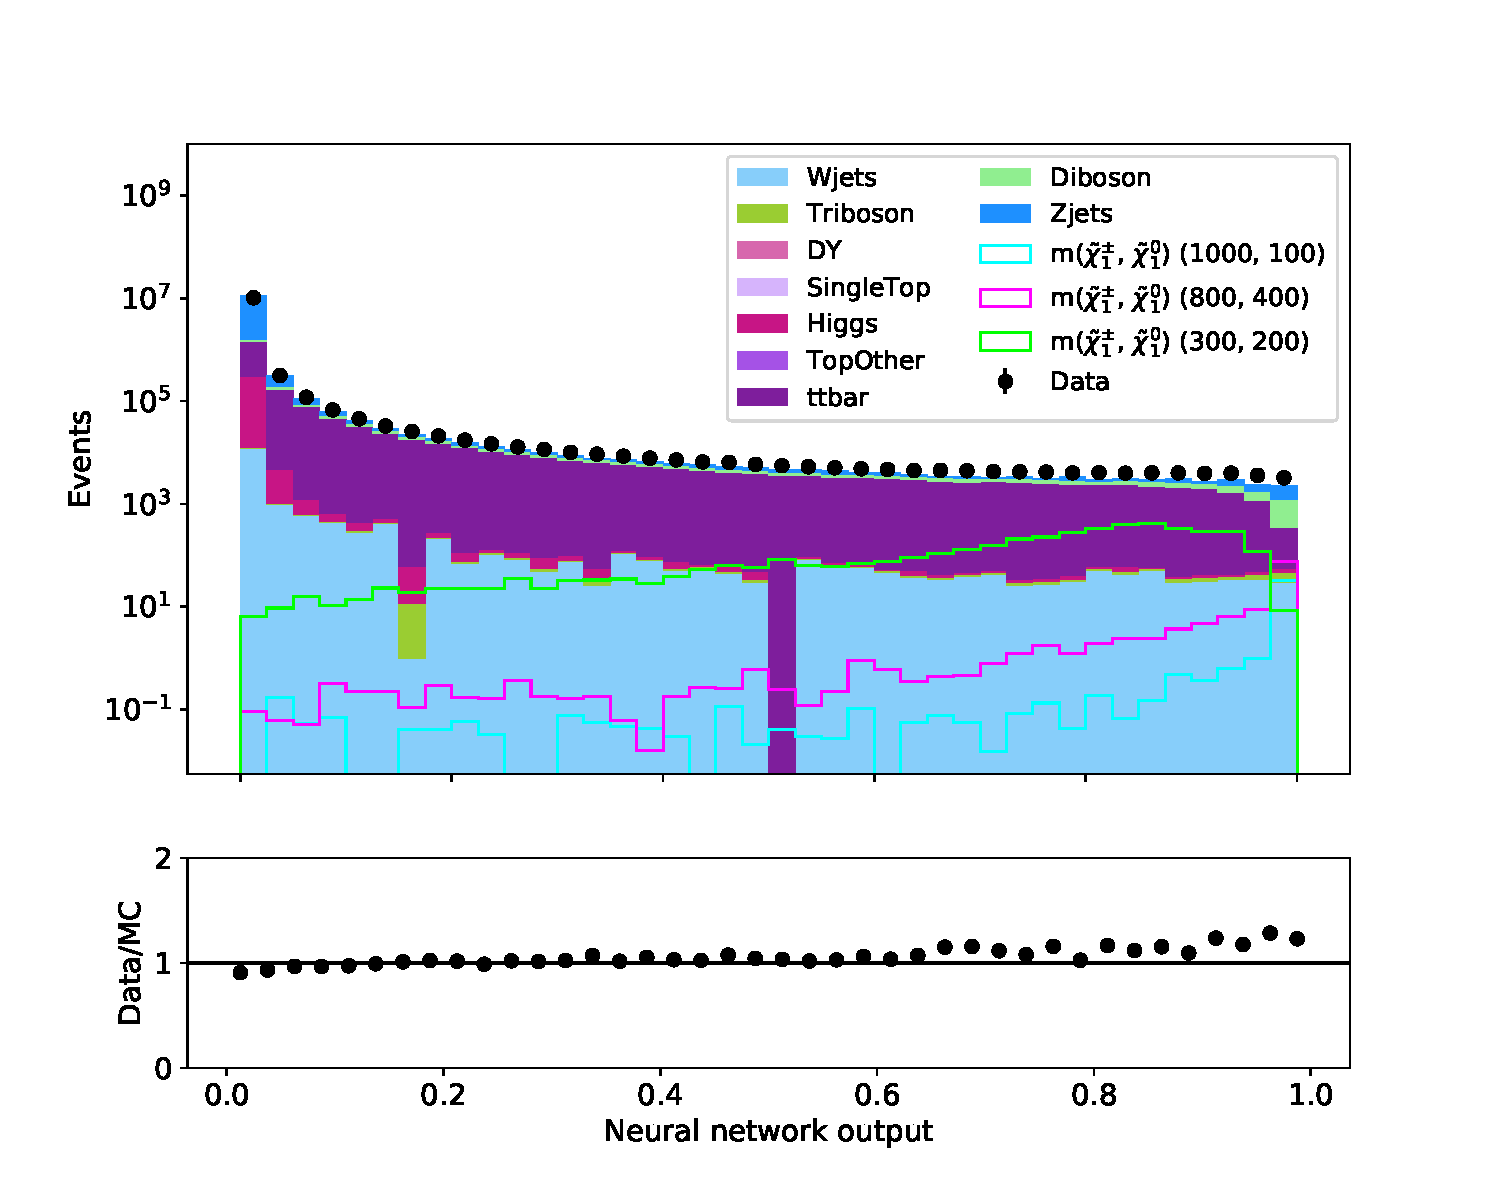
\includegraphics[width = \textwidth]{Figures/Stacked/stackedplot_NN_High_level_slepsnu.pdf}
        \caption{Chargino production via $\Tilde{l}/\Tilde{\nu}$.}
        \label{fig:}
    \end{subfigure}      
    \begin{subfigure}[t!]{0.49\textwidth}
        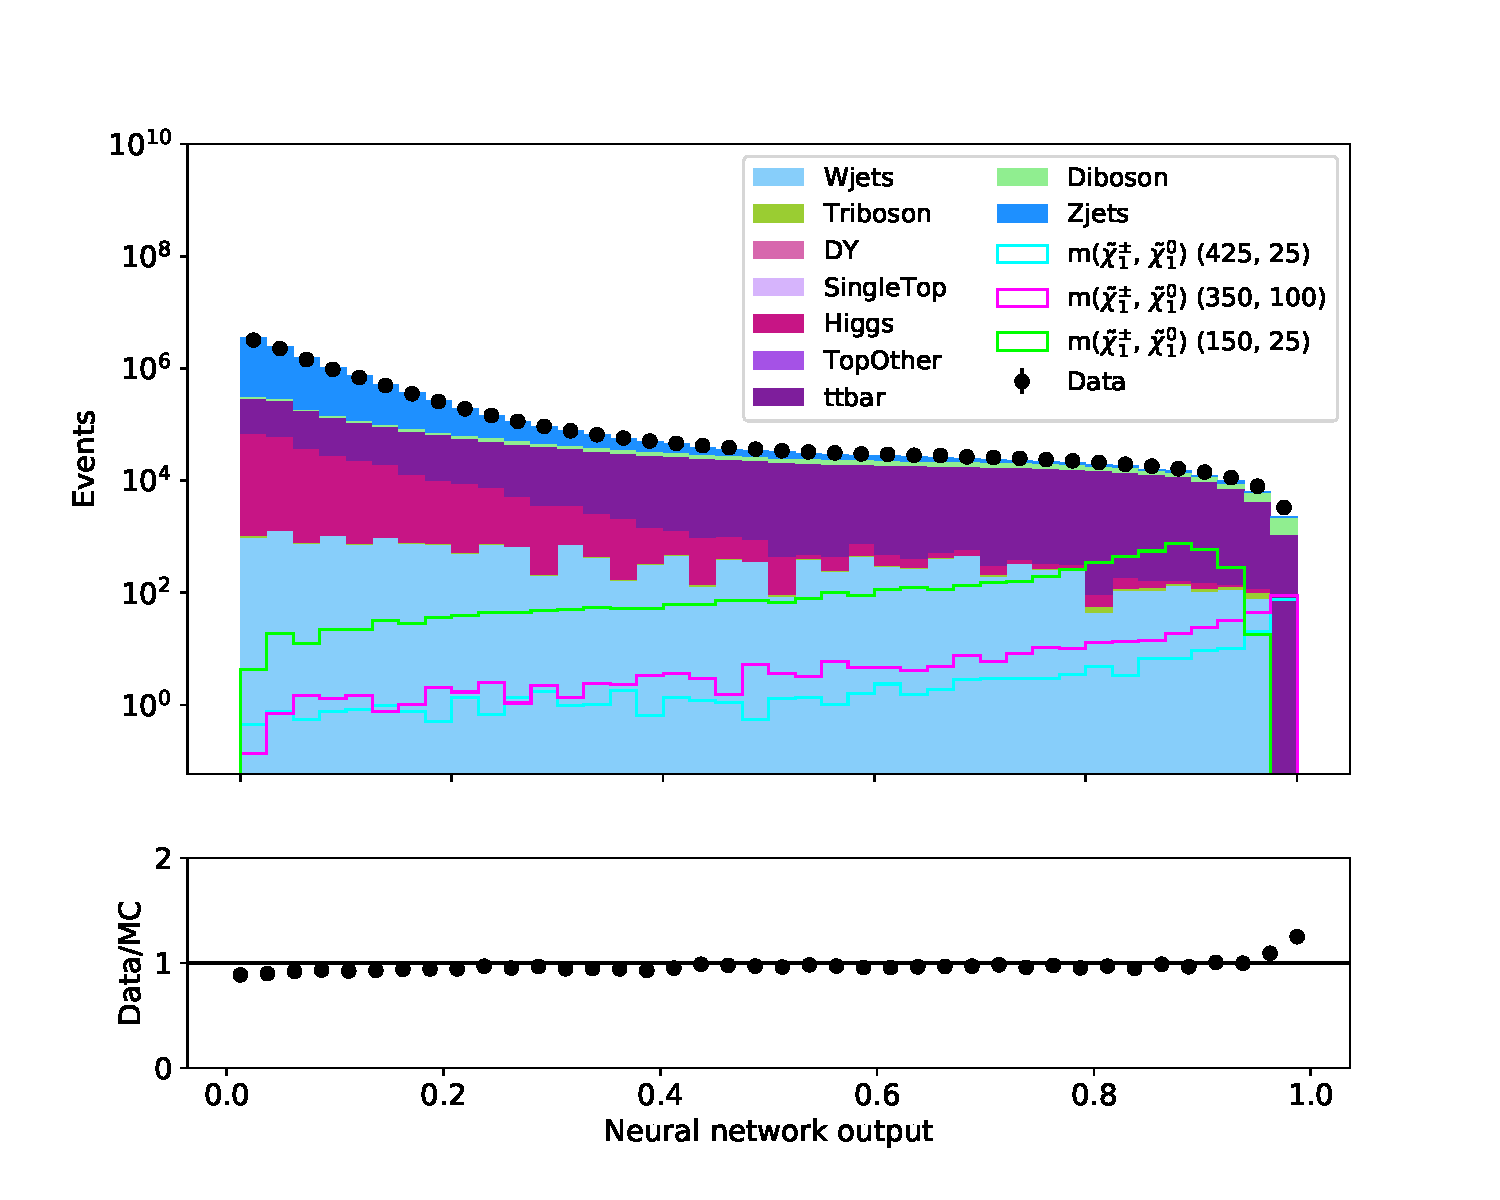
\includegraphics[width = \textwidth]{Figures/Stacked/stackedplot_NN_High_level_WW.pdf}
        \caption{Chargino production via $W^\pm$.}
        \label{fig:}
    \end{subfigure}
    \begin{subfigure}[t!]{0.49\textwidth}
        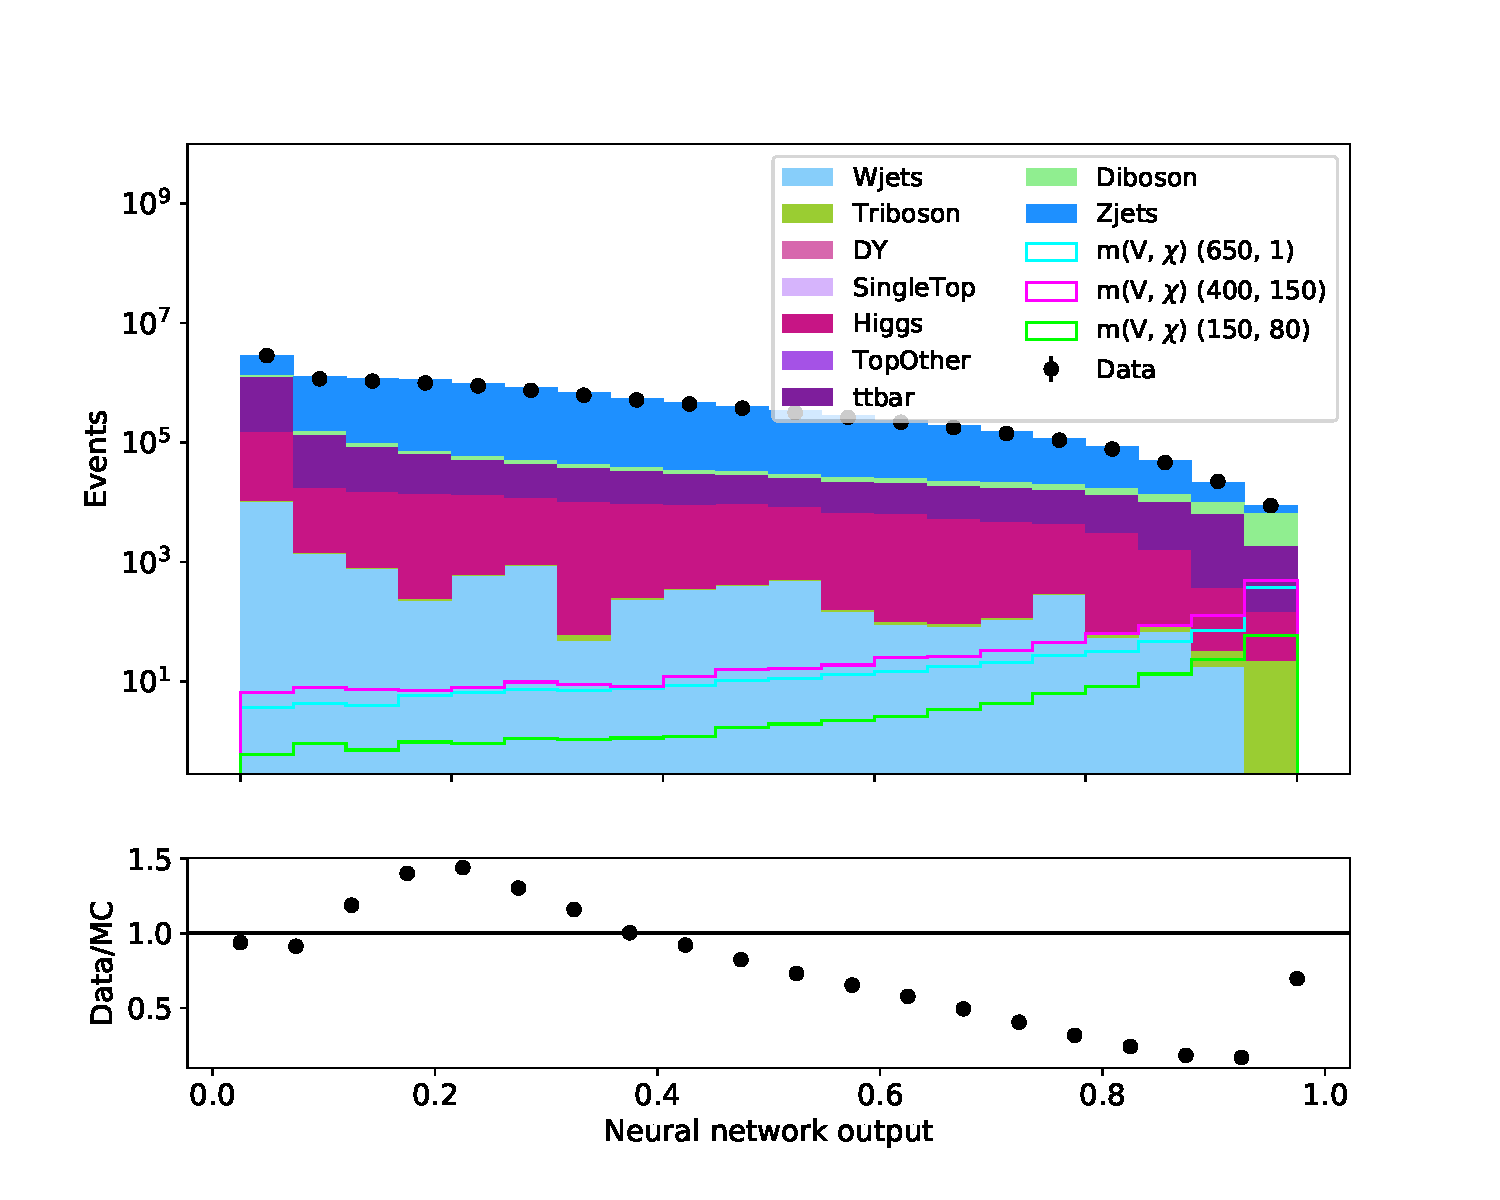
\includegraphics[width = \textwidth]{Figures/Stacked/stackedplot_NN_High_level_monoZ.pdf}
        \caption{Mono-Z.}
        \label{fig:}
    \end{subfigure}
    \caption{Test vs train for low mass splittings done with the NN using high level features during training. Here the test set is scaled up to match the number of training events.}
    \label{fig:}
\end{figure}

